\subsection{A pre-merge audit}\label{subsec:audit}

Everything in \S\ref{sec:collapse} is computed from the adapter weights, so
the regime of a cohort can be read before any merge is attempted.
Algorithm~\ref{alg:audit} does this. It reads only the $A$ factors: no $B$
factors, no base weights, no forward passes and no data. Its cost is
$O(T^2 r^2 d)$ per layer, about one CPU minute for four rank-$16$ adapters
over eight layers. We fixed the thresholds before measuring any public cohort
and use them unchanged throughout.

\begin{algorithm}[t]
\caption{Pre-merge audit of a LoRA cohort.}
\label{alg:audit}
\begin{algorithmic}[1]
\Require adapters $\{A_t\}_{t=1}^{T}$ on a common base; a sample of layers
  $\mathcal{L}$; thresholds $c_{\mathrm{hi}} = 0.9$, $c_{\mathrm{lo}} = 0.5$
\For{each pair $i < j$}
  \For{each layer $\ell \in \mathcal{L}$}
    \State $V_t \gets \mathrm{orth}\bigl(A_t^{(\ell)\top}\bigr)$ for $t \in \{i, j\}$
      \Comment{orthonormal basis of the row space}
    \State $c_{ij}^{(\ell)} \gets \operatorname{median}\,
      \operatorname{svals}\bigl(V_i^{\top} V_j\bigr)$
      \Comment{cosines of the principal angles}
  \EndFor
  \State $c_{ij} \gets \operatorname{median}_{\ell}\, c_{ij}^{(\ell)}$
\EndFor
\State $c^\star \gets \max_{i<j} c_{ij}$;\quad
  $n_{\mathrm{c}} \gets \#\{(i,j) : c_{ij} > c_{\mathrm{hi}}\}$
\State \Return \textsc{collapsed} if $c^\star > c_{\mathrm{hi}}$,
  \textsc{separated} if $c^\star < c_{\mathrm{lo}}$, else
  \textsc{indeterminate}; and $n_{\mathrm{c}}$
\end{algorithmic}
\end{algorithm}

\paragraph{Why the most similar pair.} The first version of the audit pooled
every principal cosine of every pair and took the median. The public cohorts
were sampled and first scored under that version. A registered experiment
showed that it misses a partial collapse. On each base we built a cohort of
four adapters in which only one pair of the six shares an initialisation: the
GSM8K and code adapters of a shared cohort, together with the instruction and
translation adapters of an independent one. The pooled median is $0.047$ to
$0.053$, so the old audit calls the cohort separated, while the collapsed pair
sits at $0.993$ to $0.996$. One pair is enough to break a solver. Adapter-only
RegMean at $\lambda = 10^{-6}$ leaves a worst-task excess of $0.45$ to $10.5$
nats on these cohorts, against $0.026$ to $0.155$ on the fully independent
ones, and $\kappa(\bar H)$ is $1.7\times10^{3}$ to $5.3\times10^{3}$, against
$1.5$ to $1.7$ (Table~\ref{tab:appC-hetero}). The registered consequence was to change the statistic to the maximum
over pairs, keep the thresholds, and re-read the public cohorts, which
\S\ref{subsec:public} reports. The audit also returns the number of collapsed
pairs, which says how much of a cohort is affected.

A cohort cannot be repaired by editing its $A$ factors while keeping each
adapter's behaviour. Replacing $A_t$ by $QA_t$ for an invertible $Q$, such as a permutation of the
rank dimension, keeps the
adapter the same only if $B_t$ becomes $B_tQ^{-1}$. The row space, the
principal cosines and $\bar H$ are then all unchanged. The geometry is a
property of what the adapters compute, so only retraining or the choice of
merge can change what it does to a merge.

\subsection{Which fine-tuning stacks produce the collapse}\label{subsec:libraries}

Library code decides whether two adapters receive the same initial $A$, so we
read it. In PEFT (version 0.19.1, which wrote all our adapters), the default
initialisation draws $A$ with \texttt{kaiming\_uniform\_} from the global
PyTorch generator. PEFT takes no per-adapter seed and does not reseed. Two runs
therefore receive identical $A$ exactly when the generator is in the same
state as each layer is built. That requires the same seed set beforehand, the
same target modules in the same order at the same rank, and the same device
and data type. Nothing about the task or the data enters.

The question is then what runs before the adapter is created. We read two
widely used fine-tuning stacks at pinned versions. Unsloth~\citep{unsloth2026}
(2026.5.2) gives \texttt{get\_peft\_model} a default \texttt{random\_state} of
$3407$ and sets the seed with it before creating the LoRA layers.
LLaMA-Factory~\citep{zheng2024llamafactory} sets the training seed, $42$ by
default, before the model is loaded. At their defaults, both stacks therefore
give every run on one base, target set and rank the same initial $A$. A user
who fine-tunes several tasks without changing the seed obtains a collapsed
cohort. TRL's \texttt{SFTTrainer} builds the PEFT model before it seeds, so its
behaviour depends on the calling script. We found no seeding before adapter
creation in axolotl. Without any seed the regime does not arise by accident,
since fresh processes start the generator differently. Our measurements of
both stacks agree (\S\ref{subsec:routes}).

\subsection{Prevalence in public adapters}\label{subsec:public}

Our own cohorts say nothing about anyone else's. We therefore ran the audit on
public cohorts, under a protocol registered before any adapter was downloaded.
We walked the HuggingFace model index, filtered to PEFT and sorted by
downloads, which weights the sample towards adapters that are used. We grouped
adapters into cohorts by publisher and base model. A cohort entered if it had
at least two readable LoRA adapters of rank at least $4$ on one base, sharing a
target module. Every criterion was checked from metadata before any weight was
fetched, and no cohort was skipped after inspection. We walked $1000$ models to
reach the registered $50$ cohorts. Five could not be scored, which left $45$.

\begin{figure}[pos=tbp]
\centering
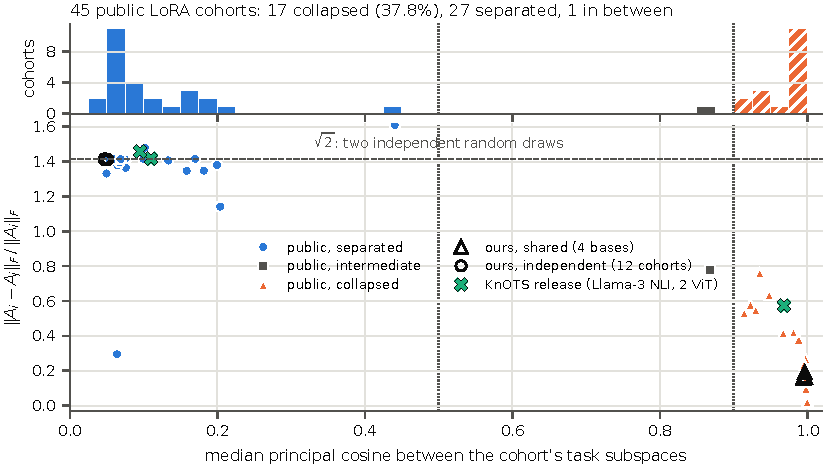
\includegraphics[width=\textwidth]{nc/figures/fig3_prevalence.pdf}
\caption{The $45$ public LoRA cohorts, sampled by a frame registered before
any download. Horizontal axis: median principal cosine between the cohort's
task subspaces, the audit statistic at the time of sampling, with the
thresholds dotted and its histogram on top. The maximum pairwise cosine of
Algorithm~\ref{alg:audit} moves two cohorts upwards (text).
Vertical axis: relative distance between the cohorts' $A$ factors, which is
$\sqrt 2$ for two independent random draws. Two cohorts whose members differ in
rank have no distance and appear only in the histogram. Open markers are our
own cohorts. Crosses are the three cohorts released with KnOTS, the one merging
paper among $22$ checked that releases LoRA cohorts.}
\label{fig:prevalence}
\end{figure}

Under the pooled median, the statistic registered at the time, $17$ of the $45$
cohorts ($37.8\%$) are collapsed. The registered prediction was at least
$20\%$. The distribution has two clear modes rather than being a continuum cut
by a threshold (Figure~\ref{fig:prevalence}): $27$ cohorts are separated, with
median cosine $0.076$, and only one falls between the thresholds, at $0.868$.
An unplanned check supports the measurement. If two adapters draw $A$
independently and $A$ moves little, then
$\|A_i - A_j\|_F \approx \sqrt2\,\|A_i\|_F$. The separated cohorts give a
median ratio of $1.414$, as independent draws should, and the collapsed
ones range from $0.017$ to $0.760$ (Figure~\ref{fig:prevalence}, vertical
axis). One separated cohort sits at only $0.29$, the single point this check
does not explain.

We re-read the cohorts under the maximum pairwise cosine about two months
after the original download. Five could no longer be read, because eleven of
their adapters had been deleted or made private; for the other $40$, the
pooled median reproduces the stored value to within $0.003$. Two statuses
change, both upwards: one cohort, with a pooled median of $0.064$ but four of
its ten pairs collapsed, becomes collapsed, and another becomes
indeterminate. No collapsed cohort leaves the class. Counting the five
unreadable cohorts at their stored status, $18$ of the $45$ ($40.0\%$) are
collapsed under the audit as it now stands, or $19$ if one unreadable cohort
of four adapters hides a collapsed pair.

\paragraph{What the collapsed cohorts are.} The sampling frame groups adapters
by publisher and base model, and such a group is not necessarily a set of
tasks anyone would merge. We read the names, model cards, tags and
configurations of the $18$ collapsed cohorts, in a reading that was not
registered. We classified each by the most specific evidence it offers of how
its members came to share $A$. In one, the card states that one adapter was
trained on top of the other, and in another that the runs used the same seed.
Four are checkpoints, stages or variants of one run, three carry the tags of
Unsloth, which seeds by default (\S\ref{subsec:libraries}), and nine are
sibling adapters with nothing recorded about seeds. None uses a non-random initialisation or shares or
freezes $A$ by design. Six cohorts hold adapters for distinct tasks that one
might merge, among them LoRAHub's $196$ FLAN-task
adapters~\citep{huang2024lorahub}, released to be composed. The other twelve
are versions, stages, checkpoints or data ablations of one model, for which
merging is rarely the point. The $40\%$ is therefore the prevalence of the
regime among public cohorts as the frame defines them, not among cohorts
built for merging, but six collapsed cohorts of distinct tasks show that the
regime is not confined to our own experiments.

The cohorts that merging papers evaluate on are harder to sample. We checked
the $22$ merging papers we cite in order, intending to audit the first two that
release LoRA cohorts, and only one does. KnOTS~\citep{stoica2025knots} releases
a Llama-3-8B cohort of six natural-language-inference adapters and two vision
cohorts. Its language cohort is collapsed, at median cosine $0.968$, and its
vision cohorts are separated, at $0.110$ and $0.095$. A later merging paper
uses this released cohort as its benchmark~\citep{panariello2025core}, so that
benchmark is in the collapsed regime. This is a single paper, so we draw no
conclusion about merging benchmarks in general.
